% create on 2016-03-14,the third chapter of thesis: Fixed-rank PSD流形判别学习方法
\chapter{低秩对称半正定矩阵判别学习方法}
\label{chap:PSD_discrim_learning}
前面的章节已经提到,统计建模图像集合的方法中有相当一部分的模型都是与样本协方差矩阵有关,但样本协方差矩阵的计算中一个很现实的问题是样本数往往小于数据维度,因为即使是$20\times 20$的小图像也有400维,也就是说至少需要400个样本才有可能使得样本协方差矩阵是非奇异的;这不管是对多视角图像的图片集合还是对视频监控(400帧的图像在30FPS的帧率下也需要13秒还多)中的视频都是很苛刻的要求。因此实际中获得的样本协方差矩阵实际上是对称半正定(Positive Semi-Definite, PSD)矩阵。在使用样本协方差矩阵建模图像集合的方法中,针对该问题的一个常用的trick是给样本协方差矩阵的对角线上加上一个正则项(如\ref{sec:Database_SPD_Construct}中介绍的一样);但是这并没从本质上解决样本协方差矩阵奇异的问题,这促使本文回到数据所在的原始集合——对称半正定矩阵集合中研究图像集合的建模和判别学习问题。

%注意到,虽然原始的对称半正定(PSD)矩阵空间是一个凸集合,但是以目前了解到的情况而言,无约束的对称半正定集合上并没有很好的定义的数学结构,与之最接近的一个数学结构是Fixed-Rank PSD集合(公式\ref{Fixed-Rank-PSD-set}),这也是我们早期的主要研究对象。
%\begin{equation}
%\label{Fixed-Rank-PSD-set}
%\mathbb{S}_{d}^{+}(k)=\{A|A\in \mathbb{R}^{n \times n},A=A^{T},\langle Ax,x\rangle \geq 0,\forall x \in \mathbb{R}^n;{\rm rank}(A)=k\}
%\end{equation}
%如果在该结构上定义合适的黎曼度量的话就可以使得该集合形成一个黎曼流形结构\cite{PSD_Riemannian};
另一方面,当使用对称正定矩阵表示图像集合的时候,对称正定矩阵的维度往往非常高,如$20 \times 20$的图像组成的集合,它的样本协方差将达到$400\times 400$的规模,这对存储和计算都是不小的负担,因此\cite{Statistics_SPDML,Statistics_LEML}研究了对称正定矩阵流形的降维问题;而不难发现的是当图像集合使用的对称半正定矩阵表示且要求矩阵的秩(Rank)很低的时候对称半正定矩阵表示将体现出另一个重要的性质:低秩(Low-Rank)。低秩的性质将大大的降低存储容量和计算时间,因为如果将对称半正定矩阵$C$进行$C=WW^{T},W \in \mathbb{R}^{d\times k},{\rm rank}(W)\leq k \ll d$分解,此时只需要存储$W$即可,这将大节省存储空间和计算量,而这正是我们想要的。

最后,回顾图像集合建模的两大分支:子空间的方法(如\cite{Subspace_GDA,Subspace_MSM}等)和统计模型建模的方法(如\cite{Statistics_CDL,Statistics_Vemu,Statistics_SPDML,Statistics_LMKML,Statistics_HERML,Statistics_DARG}等),可以发现如下事实:对于样本协方差矩阵$C_{i}$,及其特征分解$C_{i}=U_{i}\Lambda_{i} U^{T}_{i}$;子空间的方法只用到了$U_{i}$的信息,还有尺度(特征值)的信息没有被使用;而统计模型的方法使用了整个协方差矩阵的信息,但是只有很少的文章考虑了数据中的噪声和样本稀疏带来的估计不准的问题,而因此可能导致模型不够鲁棒的问题。最后反观低秩对称半正定矩阵表示中当$k<d$的时候,它更像是两者的中间状态,兼顾了两者的优点。
\begin{figure}[hbt]
	\centering
	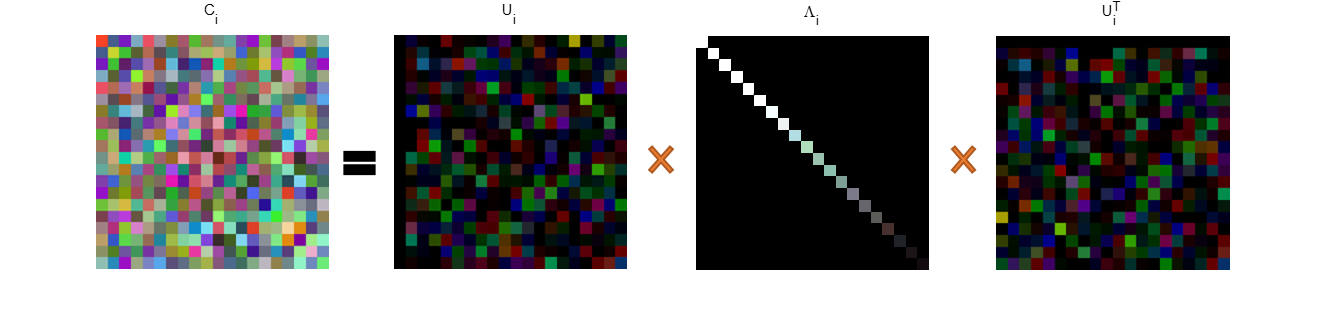
\includegraphics[width=0.95\linewidth]{source/svd_decomposition.png}
	\caption{奇异值分解示意图}
	\label{fig:SVD_Decomposition}
\end{figure}

接下来内容大致安排如下:首先结合着前期关于固定秩对称半正定矩阵流形的研究,对与低秩对称半正定(Low-Rank symmetric Positive Semi-Definite, Low-Rank PSD)矩阵关系最密切的固定秩对称半正定(Fixed-Rank symmetric Positive Semi-Definite, Fixed-Rank PSD)矩阵流形进行介绍,其中为了介绍Fixed-Rank PSD矩阵流形还会用一些篇幅简要介绍一下Stiefel Manifold和Grassmann Manifold;然后结合着工作\cite{PSD_WACV}针对Fixed-Rank PSD矩阵流形建模图像集合中存在的一些问题以及Low-Rank PSD矩阵表示图像集合的优势提出了Low-Rank PSD矩阵建模图像集合的方法;接着是Low-Rank PSD矩阵图像集合表示下的PSD编码和判别学习方法,最后是实验验证本章所提方法和以及本章内容的总结与展望。

\section{施蒂费尔流形和格拉斯曼流形}
\label{sec:Grassmann_Manifold}
这部分会对对称正定矩阵流形以外的两种流形进行介绍,分别是施蒂费尔(Stiefel)流形和格拉斯曼(Grassmann)流形,这里之所以同时介绍这两种流形主要是出于以下考虑:其一是因为Grassmann与Stiefel流形的关系密切使得两者需要同时介绍,其二是为Fixed-Rank PSD流形的介绍做准备。本节的内容只是对Stiefel流形和Grassmann流形的简要介绍,更多关于Grassmann流形以及两者的关系的内容可以参看文献\cite{Grassmann}。以下的内容以基本定义居多,但相较于\ref{sec:Manifold_SPD}节的内容这里的内容相对简单一些;接下来就首先从Grassmann流形的定义开始。
\begin{definition}
\label{Grassmann_def}
{\heiti (\textbf{Grassmann}流形)}Grassmann流形是定义在$\mathbb{R}^n$中所有$k$维的线性子空间构成的集合上的数学结构。
\begin{equation}
{\rm Gr}(k,n)=\{\mathbb{V} \subset \mathbb{R}^n,\mathbb{V}\text{ is a linear subspace with }\rm{dim}\mathbb{V}=k\}
\end{equation}
\end{definition}
当为其定义拓扑结构之后,即可构成流形结构,进一步的可以在其上导出黎曼度量\cite{Grassmann},所以它是黎曼流形的特例。我们最终希望借助Grassmann流形和对称正定矩阵流形来表示固定秩对称半正定矩阵流形,为此需要了解Grassmann流形的数学表示,而Grassmann流形的表示又借助于Stiefel流形,所以出于数学表示的方便性的考虑,这里先对Stiefel流形进行介绍。
\begin{definition}
\label{Stiefel_nonCompact_def}
{\heiti (\textbf{Stiefel(non-compact)}流形)} non-compact Stiefel流形\footnote{以下所说的流形均指集合上定义了拓扑结构的流形,为简洁起见文中仅以集合代替,而不细说拓扑结构}是定义在所有$n\times k,(0<k<n)$满秩矩阵构成的集合上的流形结构。
\begin{equation}
\begin{split}
{\rm St}(k,n)&=\{A \in \mathbb{R}^{n\times k};{\rm rank}(A)=k\}\\
&=\{A=(a_1,...,a_k)\in \mathbb{R}^{n\times k}; a_1,...,a_k \text{ are linearly independent}\}
\end{split}
\end{equation}
\end{definition}
\begin{definition}
\label{Stiefel_Compact_def}
{\heiti (\textbf{Stiefel(compact)}流形)}当在non-compact Stiefel流形\footnotemark[\value{footnote}]的定义域中要求$A$的列向量是正交的(即:$A^{T}A=I_k$)时候,即构成了compact Stiefel流形定义的集合。
\begin{equation}
{\rm St}^{*}(k,n)=\{A\in\mathbb{R}^{n\times k};A^{T}A=I_k\}
\end{equation}
\end{definition}
这里再给出一个在数学中非常重要的概念:“广义线性群(General Linear Group, GL)”,在矩阵流形的研究中将常常见到它的身影。
\begin{definition}
\label{General_Linear_Group}
{\heiti (广义线性群(\textbf{General Linear Group}))}在数学中对于指定的$n$将所有$n\times n$的可逆矩阵的集合称为广义线性群,并记为:
\begin{equation}
{\rm GL}(n)=\{A \in \mathbb{R}^{n\times n};{\rm{det}}(A)\neq 0\}
\end{equation}
\end{definition}

至此,介绍Grassmann流形的准备工作已基本完成,接下来将利用这些定义以及\ref{sec:manifold_Riemaniann}节的内容对Grassmann流形的数学表示进行介绍。为此这里先来捋一捋Grassmann流形和Stiefel流形的关系:
\begin{rela}
\label{Relation_SS}
{\heiti (\textbf{Stiefel(non-compact) V.S Stiefel(compact)})}定义${\rm GS}(\cdot)$表示Gram-Schmidt正交化变换,于是\begin{equation}
{\rm GS}:{\rm St}(k,n) \rightarrow {\rm St}^{*}(k,n)
\end{equation}
\end{rela}
显然${\rm GS}(\cdot)$变换是满射但是不是入射所以${\rm GS}(\cdot)$不是一一的映射。
\begin{rela}
\label{psd_map_pi}
{\heiti (\textbf{Stiefel(non-compact) V.S Grassmann})}定义如公式\ref{noncSt2Gr}所示的变换$\pi$描述两者之间的关系。
\begin{equation}
\label{noncSt2Gr}
\pi:{\rm St}(k,n) \rightarrow {\rm Gr}(k,n),A=(a_1,...a_k)\rightarrow {\rm{span}}(A)
\end{equation}
\end{rela}
同样的$\pi$只是满射但是不是入射,关于映射$\pi$的还有一些性质需要了解:
\begin{itemize}
\item 首先已知$\pi$是满射,对于任意的矩阵$A \in St(k,n)$有
\begin{equation}
\pi^{-1}[\pi(A)]=\{AP;P\in {\rm GL}(k)\}
\end{equation}
\item 映射$\pi$是连续(continuous)的开(open)的(开(open)的意思是说映射的像是开集的话原像也是开集)
\end{itemize}
\begin{rela}
{\heiti (\textbf{Stiefel(compact) V.S Grassmann})}类似于关系\ref{psd_map_pi},定义Stiefel(compact) 和 Grassmann之间的映射$\bar{\pi}$\ref{cSt2Gr}。
\begin{equation}
\label{cSt2Gr}
\bar{\pi}:{\rm St}^{*}(k,n)\rightarrow {\rm Gr}(k,n);A=(a_1,...,a_k)\rightarrow {\rm{span}}(A),A^{T}A=I_k 
\end{equation}
\end{rela}
不难发现映射$\bar{\pi}$与$\pi$之间存在如下的关系:$\pi=\bar{\pi}\circ {\rm GS}$。

前面给出了诸多定义和关系,其目的主要是为了给出Grassmann流形的一个数学表示,方便对其进行研究和应用。
\begin{repr}
\label{non-compact-repr}
利用non-compact Stiefel流形将Grassmann流形表示为如下的商空间(quotient space)的形式
\begin{equation}
St(k,n)/GL(k,\mathbb{R})=\{[A]|[A]\triangleq A[GL(k)];A\in St(k,n)\}
\end{equation}
\end{repr}
\begin{repr}
\label{compact-repr}
Grassmann流形也可利用商空间的概念使用compact Stiefel流形表示:
\begin{equation}
\begin{split}
{\rm St}^{*}(k,n)/{\mathcal{O}}(k)&=\{[A]|[A]\triangleq A[\mathcal{O}(k)];A\in {\rm St}^{*}(k,n\}\\
\mathcal{O}(k)&=\{U|U\in \mathbb{R}^{k\times k};U^{T}U=I_k\}
\end{split}
\end{equation}
\end{repr}
在两种表示中,第二种表示方法更为常用,对该表示的研究也相对成熟一些。在这一小节的最后将介绍Grassmann流形上的度量表示。为此来先介绍两个基本概念:“主夹角”和“投影变换”。
\begin{definition}
\label{Principle_Angle}
{\heiti (主夹角)}假定$X_1,X_2,\in {\rm St}^{*}(k,\mathbb{R}^{n})$表示两个子空间的基矩阵,定义子空间$V_1={\rm{span}}(X_1),V_2={\rm{span}}(X_2)$之间的主夹角为:
\begin{equation}
\begin{split}
\cos\theta_i&=\max_{\bm{u}_i\in V_1}\max_{\bm{v}_i \in V_2}\bm{u}_{i}^{T}\bm{v}_i\\
s.t~~~~& \bm{u}_{i}^{T}\bm{u}_i=1,\bm{v}_{i}^{T}\bm{v}_i=1\\
~~~& \bm{u}_{i}^{T}\bm{u}_j=0,\bm{v}_{i}^{T}\bm{v}_j=0;j \leq i
\end{split}
\end{equation}
其中的$\theta_i,i=1,2,...,k$称为主夹角。
\end{definition}
\begin{definition}
\label{Projection}
{\heiti (投影变换)}在$\mathbb{R}^{n}$空间中,设$S_k$是其中的一个子空间,并且$U$是子空间中的基矩阵($n \times k$),则$\mathbb{R}^{n}$到$S_k$中的投影算子表示如\ref{Projection_Operator}所示。
\begin{equation}
\label{Projection_Operator}
\Pi_k:U\rightarrow UU^{T};U \in {\rm St}^*(k,\mathbb{R}^n)\text{ and }UU^{T} \in \mathbb{S}_n
\end{equation}
\end{definition}
其中$\mathbb{S}_n$表示的是对称矩阵构成的空间。实际上,投影矩阵$UU^{T}$是半正定的。利用“主夹角”和“投影变换”两个概念可方便的介绍Grassmann流形上两个常用的度量的:“投影度量”和“比奈-柯西度量”
\begin{definition}
\label{Projection_metric}
{\heiti (投影度量)}假定$X_1,X_2,\in {\rm St}^{*}(k,\mathbb{R}^{n})$表示两个子空间的基矩阵,并且有主夹角$\{\theta_i\}_{i=1}^{k}$,两者之间定义投影距离度量的定义如\ref{proj_dist}所示。
\begin{equation}
\label{proj_dist}
d(X_1,X_2)=\|\Pi_k(X_1)-\Pi_k(X_2)\|_{2}=\left(\sum_{i=1}^{k}\sin^{2}(\theta_i)\right)^{\frac{1}{2}}
\end{equation}
\end{definition}
其中的$\Pi_k(\cdot)$就是前面的投影变换,这也是“投影度量”的由来。
\begin{definition}
\label{BC_metric}
{\heiti (比奈-柯西度量)}利用主夹角的cosine值$\{\cos(\theta_i)\}_{i=1}^{k}$将该度量定义如下:
\begin{equation}
d(X_1,X_2)=\left(1-\Pi_{i=1}^{k}\cos^{2}(\theta_i)\right)^{1/2}
\end{equation}
\end{definition}
以上是本文关于Grassmann流形的简要介绍,更多关于Grassmann流形的内容可以参看文献\cite{Grassmann},里面有更加详细的介绍,但是可能会比较晦涩。
\section{固定秩对称半正定矩阵流形}
\label{sec:Fixed-rank-PSD}
本文用$\mathbb{S}_{d}^{+}(k)$表示$d \times d$秩为$k$的半正定矩阵组成的集合,它也是我们前期的主要研究对象。接下来将会对固定秩的对称半正定矩阵(Low-Rank symmetric Positive Semi-Definite, PSD)流形的Geomentry结构做简要的介绍,主要内容参考\cite{PSD_Riemannian}。

对于任意的元素$A \in \mathbb{S}_{d}^{+}(k)$将其分解为$A=UR^2U^{T},U\in St^{*}(k,d),R \in \mathbb{S}_{k}^{+}$则这里给出如公式\ref{psd_svd}所示的形式。
\begin{equation}
\label{psd_svd}
A=UR^2U^{T}=(UR)(UR)^{T} \triangleq ZZ^{T};Z \in {\rm St}(k,d)
\end{equation}
这里注意到对任意的正交阵$O \in \mathcal{O}(k)$有$(ZO)(ZO)^{T}=ZZ^{T}$表示的是同一个半正定矩阵因此定义如下的关系:
\begin{equation}
\label{map_by_ortho}
\begin{split}
&R \sim O^{T}RO \in \mathbb{S}^{+}_{k}\\
&U \sim UO \in {\rm St}^{*}(k,d)\\
&ZO=URO \sim UOO^{T}RO
\end{split}
\end{equation}
其中$\sim$表示等价关系,最后定义如下的直积的形式来表示对称半正定的矩阵。
\begin{equation}
\label{psd_product}
(U,R^2)\sim (UO,O^{T}R^2O) \in {\rm St}^*(k,d)\times \mathbb{S}^{+}_{k}
\end{equation}
运用上述公式的内容来表示固定秩半正定矩阵$A$的时候,在其切空间$T_A\mathbb{S}_{d}^{+}(k)$处的无穷小变量$(\Delta,D)$定义为(具体形式可参看文献\cite{PSD_Riemannian}):
\begin{equation}
\label{psd_varation}
\begin{split}
&\Delta=U_{\perp}B,\\
&D=RD_{0}R,\\
\end{split}
\end{equation}
其中$U_{\perp} \in {\rm St}^{*}(d-k,d),U^{T}U_{\perp}=\bm{0};B \in R^{(d-k)\times d}$,而$D_0 \in \mathbb{S}_d$。有了以上的定义后,进一步参考${\rm St}^{*}(k,d)$和$\mathbb{S}^{+}_{k}$上的黎曼度量定义两个微小变量之间的关系\ref{psd_riemannian_metric}。
\begin{equation}
\label{psd_riemannian_metric}
\begin{split}
&g_{(U,R2)}((\Delta_1,D_1), (\Delta_2,D_2)) \\
&~~~~~~~~= {\rm tr}(\Delta_1\Delta_2)+ \lambda~{\rm tr}(R^{−1}D_1R^{−2}D_2R^{−1}),\lambda>0
\end{split}
\end{equation}
可以证明,上式定义了切空间$T_A\mathbb{S}_{d}^{+}(k)$上的黎曼度量\cite{PSD_Riemannian}。公式\ref{psd_curve}利用固定秩对称半正定矩阵中的黎曼度量公式\ref{psd_riemannian_metric}定义了固定秩对称半正定矩阵A,B之间的一条曲线。
\begin{equation}
\label{psd_curve}
\left\{
\begin{aligned}
&let:A\sim(U_A,R_{A}^{2}),B\sim(U_B,R_{B}^{2})\\
&PA\text{ of }U_A,U_B:\Theta={\rm diag}(\theta_1,\theta_2,...,\theta_k)\\
&part1:U(t)=U_A\cos(\Theta t)+X\sin(\Theta t)\\
&part2:R^2(t)=R_{A}\exp\left(t\log\left(R_{A}^{-1}R_{B}^{2}R_{A}^{-1}\right)\right)R_{A}\\
&curve:\gamma_{A \rightarrow B}(t)=U(t)R^{2}(t)U(t)^{T}\\
&length:L(\gamma_{A \rightarrow B})=\|\Theta\|_{F}^{2}+p~\|\log\left(R_{A}^{-1}R_{B}^{2}R_{A}^{-1}\right)\|_{F}^{2}
\end{aligned}
\right.
\end{equation}
公式\ref{psd_curve}中的$PA$是Principle Angles的缩写;$X=(I-U_AU_{A}^{T})U_BF$,其中$F$是矩阵${\rm diag}(\sin(\theta_1),\sin(\theta_2),...,\sin(\theta_k))$的逆(或伪逆);而上式中的$L(\gamma_{A \rightarrow B})$给出了曲线之间的长度,根据定义\ref{Length}如果要进一步的给出流形上的测地距离则需要找到链接$A,B$所有曲线中长度最小的曲线$\gamma_{A \rightarrow B}^{*}(t)$,这对于固定秩的对称正定矩阵流形过复杂,不过好在文献\cite{PSD_Riemannian}证明的了$L(\gamma_{A \rightarrow B})$是测地距离的一个不错估计(虽然它不一定满足三角不等式),所以接下来就可以运用该“度量”。
\begin{equation}
\label{polar_metric}
\delta^{2}_{FRPSD}(A,B)=\|\Theta\|_{F}^{2}+p~\|\log\left(R_{A}^{-1}R_{B}^{2}R_{A}^{-1}\right)\|_{F}^{2}
\end{equation}
\section{固定秩对称半正定矩阵流形研究概况}
\label{sec:Fixed-Rank-PSD-Current}
本节的主要内容是介绍固定秩对称半正定(Fixed-Rank symmetric Positive Semi-Definite, Fixed-Rank PSD)矩阵流形上的判别学习方法。关于对称半正定矩阵(symmetric Positive Semi-Definite, PSD)的研究主要分为如下几个方向:比较纯粹的理论研究(如工作\cite{PSD_Riemannian,PSD_Regression}等),然后是做优化的(如半正定规划问题)研究(如工作\cite{PSD_Opt1}),再者是做度量学习的工作(如AAAI'2016的工作\cite{PSD_AAAI}),最后是做图像集合分类的工作,目前据我们所知只有发表在“Winter Conference on Applications of Computer Vision (WACV), 2016”的工作\cite{PSD_WACV},由于该工作与我们前期的研究内容非常相近并考虑到其前瞻性,接下来将简单的介绍一下,顺带介绍一下Fixed-Rank PSD流形做图像集合分类的这个分支。而其它的分支,如基础理论的已经在\ref{sec:Fixed-rank-PSD}部分做了介绍,优化与度量学习的分支将会在对工作\cite{PSD_AAAI}进行介绍的时候提及,所以这里不再赘述了,接下来就先看一下工作\cite{PSD_WACV}。

工作\cite{PSD_WACV}针对本章开头部分提到的问题,首次利用Fixed-Rank PSD矩阵建模图像集合,用于图像集合的分类问题。文中所提出的方法十分直接,遵循了解决图像集合分类问题的两个基本步骤:1.为图像集合寻找一种表示(这里选择的就是Fixed-Rank PSD矩阵);2.为这种表示寻找/推导一种度量用于描述两个集合表示的相似度/距离。
\subsection{固定秩对称半正定矩阵表示图像集合}
\label{sec:Fixed_Rank_PSD_repr_Imageset}
首先,不妨假设数据包含$n$个图像集合分别属于$C$个类别,并使用标签$y_{i}\in\{1,2,\cdots,C\},i=1,2,\cdots,n$标记(label)。每个集合有$n_i$个样本,每个样本来自$\mathbb{R}^{d}$的空间,于是将由图像集合构造Fixed-Rank PSD矩阵表示的过程描述如下(设${\rm rank}=k$):
\begin{itemize}
\label{construct_fixed_rank_PSD}
\item 设$\{\bm{x}_{ij} \in \mathbb{R}^{d}\}_{j=1}^{n_i}$表示第$i$个图像集合
\item 计算样本均值:$\bar{\bm{x}}_i=\frac{1}{n_i}\sum_{i=1}^{n_i} \bm{x}_{ij}$,样本协方差:$C_i=\frac{1}{n_i-1}\sum_{j=1}^{n_i}(\bm{x}_{ij}-\bar{\bm{x}}_i)(\bm{x}_{ij}-\bar{\bm{x}}_i)^{T}$
\item 对样本协方差矩阵做奇异值分解获得:$C_i=U_i\Lambda_iU_{i}^{T}$,并假设分解结果按特征值由大到小排列
\item 对于给定的${\rm rank}=k$,选取$U_i$的前$k$列$Y_i=U_i(:,1:k)\in {\rm St}^{*}(d,k)$以及$\Lambda_i$的$k$阶主子式$R_{i}^{2}=\Lambda_{i}(1:k,1:k)\in \mathbb{S}_{k}^{+}$作为图像集合的Fixed-Rank PSD表示$(Y_i,R_{i}^{2})$,关于该表示具体可参看本文的\ref{sec:Fixed-rank-PSD}或参考文献\cite{PSD_Riemannian}
\end{itemize}
通过上述的步骤为每一个图像集合构造Fixed-Rank PSD矩阵的表示,为了方便理解这里使用图\ref{fig:FRPSD}对Fixed-Rank PSD进行示意,而关于奇异值分解的示意则可参看图\ref{fig:SVD_Decomposition}。
\begin{figure}[hbt]
	\centering
	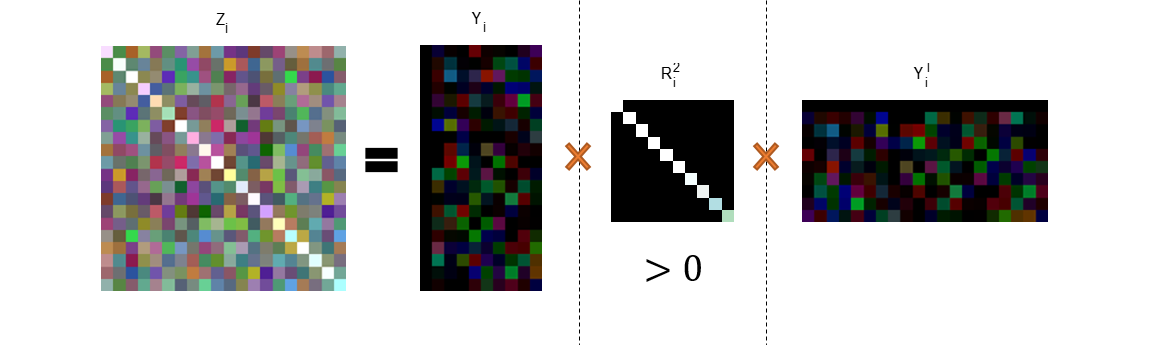
\includegraphics[width=\linewidth]{source/FRPSD.png}
	\caption{固定秩对称半正定矩阵示意图}
	\label{fig:FRPSD}
\end{figure}\\
接下来的部分将借助这种表示对图像集合的分类问题做进一步的探索。
\subsection{固定秩对称半正定矩阵流形用于图像集合分类}
\label{sec:Fixed-Rank-PSD-ImageSet-Start}
在\ref{sec:Fixed_Rank_PSD_repr_Imageset}一节根据\cite{PSD_Riemannian}中介绍的Fixed-Rank PSD矩阵流形的geometry结构对图像集合$i$使用了$(Y_i,R_{i}^{2})\in Gr(n,k)\times \mathbb{S}_{d}^{+}$的表示,使用该表示并运用公式\ref{polar_metric}定义的$\delta_{FRPSD}(\cdot,\cdot)$即可进行图像集合的分类问题了,但是这样的分类方式过于粗糙,没有包含判别性、large margin等一些性质,不利于模型的推广(文献\cite{PSD_WACV}),所以参考\cite{Subspace_GDA,Statistics_CDL}等工作以及工作\cite{Kernel_Riemannian,Dictionary_Extrinsic_method}关于黎曼流形上正定核的结论,也可以为Fixed-Rank PSD矩阵流形定义正定的核的形式来克服以上提到的问题。

关于Fixed-Rank PSD流形上(假设${\rm rank}=k$)的$\delta_{FRPSD}(\cdot,\cdot)$(公式\ref{polar_metric})这里还有一些事实需要注意(为了阐述的方便这里将公式\ref{psd_riemannian_metric}和公式\ref{polar_metric}糅合在一起后用不同的颜色标出前后两部分):
\begin{equation}
\label{polar_metric_split}
\left\{
\begin{aligned}
&g_{(U,R^2)}((\Delta_1,D_1), (\Delta_2,D_2)) \\
&~~~~~~~~~~~={\color{blue}\boxed{{\rm tr}(\Delta_1\Delta_2)}}+ \lambda~{\color{green}\boxed{{\rm tr}(R^{−1}D_1R^{−2}D_2R^{−1})}},\lambda>0\\
&\delta^2(A,B)={\color{blue}\boxed{\|\Theta\|_{F}^{2}}}+\lambda~{\color{green}\boxed{\|\log\left(R_{A}^{-1}R_{B}^{2}R_{A}^{-1}\right)\|_{F}^{2}}}
\end{aligned}
\right.
\end{equation}

其中$\Delta_i,D_i,i=1,2;R_A,R_B,\Theta$的定义请参看\ref{sec:Fixed-rank-PSD}部分的介绍;对于公式\ref{polar_metric_split},注意到其前半部分实际上是Grassmann流形的测地距离,而它与\ref{sec:Grassmann_Manifold}部分介绍的投影度量(Projection Metric,公式\ref{proj_dist})之间仅相差一个倍数关系\cite{PSD_WACV},所以公式\ref{polar_metric_split}的前半部分可以由投影度量来代替,对于公式\ref{polar_metric_split}的后半部分,注意到这是SPD矩阵流形的AIM\cite{AIM_metric}度量,进一步的注意到$R_A,R_B$都是对角矩阵,于是可以得到:$\|\log\left(R_{A}^{-1}R_{B}^{2}R_{A}^{-1}\right)=2\|\log(R_A)-\log(R_B)\|$。综合以上两点特点$\delta^{2}(A,B)$可以进一步的形式化为:
\begin{equation}
\label{polar_metric_kernel}
\begin{split}
\delta^{2}_{FRPSD}(A,B)&=\|Y_{A}Y_{A}^{T}-Y_{B}Y_{B}^{T}\|^{2}_{F}+\lambda\|\log(R_{A})-\log(R_{B})\|^{2}_{F},\lambda>0\\
&=2k-2\|Y_{A}^{T}Y_{B}\|^{2}_{F}+\lambda\|\log(R_{A})-\log(R_{B})\|^{2}_{F}\\
\end{split}
\end{equation}
其中$Y_A,Y_B$的定义在\ref{construct_fixed_rank_PSD}部分已经给出,公式\ref{polar_metric_kernel}中定义的距离很容易证明在$\mathbb{S}^{+}_{d}(k)$上对所有的$\lambda>0$它都是负定的\cite{PSD_WACV},因此容易从\ref{polar_metric_kernel}出发构造正定的核,表格\ref{tab:psd_kernel_list}列出了文章\cite{PSD_WACV}中使用的核。
\begin{table}[htb]
  \centering
  \begin{minipage}[t]{0.8\linewidth} % 如果想在表格中使用脚注,minipage是个不错的办法
  \caption{固定秩对称半正定矩阵流形中的核}
  \label{tab:psd_kernel_list}
    \begin{tabular*}{\linewidth}{lp{10cm}}
      \toprule[1.5pt]
      {\heiti 名称} & {\heiti 形式化} \\\midrule[1pt]
      线性核 & $k_{l}(A,B)=\|Y_{A}^{T}Y_{B}\|_{F}^{2}+\lambda{\rm tr}(\log(R_A)\log(R_B))$\\
      多项式核 & $k_{p}(A,B)=\left(\beta+\|Y_{A}^{T}Y_{B}\|_{F}^{2}+\lambda{\rm tr}(\log(R_A)\log(R_B))\right)^{\alpha}$\\
      拉普拉斯核 & $k_{L}(A,B)=\exp\left(-\beta\sqrt{\lambda\|\log(R_A)-\log(R_B)\|_{F}^{2}-2\|Y_{A}^{T}Y_{B}\|_{F}^{2}}\right)$\\
      RBF核 & $k_{R}(A,B)=\exp\left(-\beta\left(\lambda\|\log(R_A)-\log(R_B)\|_{F}^{2}-2\|Y_{A}^{T}Y_{B}\|_{F}^{2}\right)\right)$\\
      \bottomrule[1.5pt]
    \end{tabular*}
  \end{minipage}
\end{table}\\
最后工作\cite{PSD_WACV}中还对比了经过核判别学习(Kernel Discriminant Analysis, KDA)与不经过KDA学习利用最近邻分类的结果;文章最终的实验在手势识别,视频人脸识别和动态纹理识别进行了验证,关于实验的细节以及结果可以从文章\cite{PSD_WACV}获得,在本章的实验部分也将对这个方法作进一步的讨论。
\section{低秩对称半正定矩阵判别学习方法}
\label{sec:Low-Rank-PSD-Discrim-Approch}
\ref{sec:Fixed-Rank-PSD-ImageSet-Start}小节结合着我们前期的一些尝试介绍了Fixed-Rank PSD矩阵流形用于图像集合分类的工作\cite{PSD_WACV};但是研究中我们发现如下问题:1)通过特征分解获得Fixed-Rank PSD表示的方法\ref{construct_fixed_rank_PSD}比较粗暴,没有考虑其它的信息(如label)的利用;2)虽然工作\cite{PSD_Riemannian}中对$\delta_{FRPSD}(\cdot,\cdot)$(公式\ref{polar_metric})的形式化过程进行了详细的推导,但是$\delta_{FRPSD}(\cdot,\cdot)$本身割裂了$Y_A,R_A$(Grassmann流形和SPD矩阵流形)之间的联系,更切确的说是$\delta_{FRPSD}(\cdot,\cdot)$仅仅借助一个平衡因子$\lambda$很难完全刻画Fixed-Rank PSD矩阵$C_A=Y_{A}R_{A}^{2}Y_{A}^{T}$的关系。

针对上述的一些问题本节给出了我们的改进方案,最后关于方法的验证会在实验部分给出;这里首先要介绍的是如何为每个图像集合构造更具判别力的PSD矩阵表示。

在Mu Yadong发表在的AAAI'16的文章\cite{PSD_AAAI}中,为了在度量学习(Metric Learning, ML)的学习过程中保证马氏距离中的度量矩阵$M$是固定秩对称半正定的以及为了加速算法,文章在固定秩的矩阵流形上提出了一种新的二阶黎曼Retraction算子\footnote{关于Retraction算子读者可以参考本文的第二章}(Second Order Riemannian Retraction Operator)。文中作者构造性的使用$Z_{i}=W_iW_{i}^{T},W_{i}=\left((C_{i}^{1/2}+Z) Y_{i}\right),Y_{i}=U_{i}(:,1:k)$构造PSD矩阵,其中$C_{i},U_{i},Y_{i}$的定义同\ref{construct_fixed_rank_PSD}部分的定义,$Z$是未知的参数,文章\cite{PSD_AAAI}通过要求$Z$满足Fixed-Rank PSD矩阵流形的切空间中的性质来获得一个好的表示,详细内容可以参看文献\cite{PSD_AAAI}。这启示我们在PSD矩阵编码图像集合的时候可以借鉴这种形式,并通过$Z$编码更多的信息,如样本的label信息。

另一方面,前面已经指出$\delta_{FRPSD}(\cdot,\cdot)$(公式\ref{polar_metric})虽然保持了很好geometry相关的性质,但是其分离的形式使得其无法很好的刻画$Y_{i}\in {\rm Gr}(n,k),R_{i} \in \mathbb{S}_{k}^{+}$之间的联系,所以需要寻找一种新的度量形式来刻画两个对称半正定矩阵之间的相似度/距离。为此,如同文章\cite{PSD_Riemannian}一样,考虑到对称半正定矩阵与对称正定矩阵之间的关联性,这里先来回顾一下对称正定矩阵流形中的不同距离度量,并期望从中获得解决方案。
\begin{table}[htb]
	\centering
	\caption{对称正定矩阵流形上的距离度量}
	\begin{tabular}{llcc}
	\toprule[1.5pt]
		{\heiti 距离度量} &{\heiti 形式化} &{\heiti 是测地距离} &{\heiti 可接受不满秩输入}\\ \hline
		Affine-Invariant度量\cite{AIM_metric} &$\|\log(X_{i}^{-\frac{1}{2}}X_jX_{i}^{-\frac{1}{2}})\|_F$ &$\surd$ &$\times$ \\
		Log-Euclidean度量\cite{LEM_metric} &$\|\log(X_{i})-\log(X_{j})\|_F$ &$\surd$ &$\times$ \\
		Stein散度\cite{Stein_divergence} &$\log{\rm det}(\frac{X_1+X_2}{2})-\frac{1}{2}\log{\rm det}(X_1X_2)$ &$\times$ &$\times$ \\
		Jeffreys散度\cite{Jeffreys_divergence} &$\frac{1}{2}{\rm tr}(X_{1}^{-1}X_2+X_{2}^{-1}X_{1})-d$ &$\times$ &$\times$\\
		Cholesky距离\cite{Cholesky_distance} &$\|chol(X_1)-chol(X_2)\|_{F}$ &$\times$ &$\surd$\\
		Power-Euclidean度量\cite{Cholesky_distance} & $\frac{1}{\alpha}\|X_{1}^{\alpha}-X_{2}^{\alpha}\|_{F}$ &$\times$ &$\surd$\\
	\bottomrule[1.5pt]
	\end{tabular}
	\label{tab:SPD_metric_list}
\end{table}\\
表格\ref{tab:SPD_metric_list}中$chol(\cdot)$表示的是Cholesky分解。

表格\ref{tab:SPD_metric_list}中列出的所有的度量均可用于对称正定矩阵的之间距离的度量,其中Affine-Invariant度量和Log-Euclidean度量分别在\cite{AIM_metric}和\cite{LEM_metric}被提出,且它们有各自的黎曼度量也是是$\mathbb{S}_{d}^{+}$上的测地距离,并且Log-Euclidean度量以其优于Affine-Invariant度量的计算性质而赢得了不少青睐,但是遗憾的是这两种度量都不能用于不满秩(也就是半正定的)的情况,Stein散度\cite{Stein_divergence}和Jeffreys散度\cite{Jeffreys_divergence}最初是为了提高计算效率而提出来的,但是由于Stein散度需要计算$\log {\rm det}(\cdot)$而Jeffreys散度需要计算$X_{i}^{-1},i=1,2$所以也不能直接用于处理半正定的输入,最后剩下Cholesky距离\cite{Cholesky_distance}和Power-Euclidean度量\cite{Cholesky_distance}这两种度量由于不涉及求逆或者$\log(\cdot)$操作所以可以直接用于半正定矩阵,而与$\delta_{FRPSD}(\cdot,\cdot)$(公式\ref{polar_metric})相比,其直接考虑半正定输入,没有割裂${\rm Gr}(d,k),\mathbb{S}_{k}^{+}$之间的关系,应该有更好的表示能力;但需要注意到的是Cholesky距离和Power-Euclidean度量并不是$\mathbb{S}_{d}^{+}$上的测地距离更不是$\mathbb{S}_{d}^{+}(k)$上的测地距离,因此不能完全刻画$\mathbb{S}_{d}^{+}(k)$的geometry的结构,不过本文相信它们的联合的形式的优点能够弥补其不是测地距离的不足(最后的实验验证了我们的观点)。接下来这里选择Cholesky距离和Power-Euclidean度量作为半正定矩阵的度量。特别地,简单的验证试验发现Power-Euclidean度量比Cholesky距离能够更好的刻画数据本身的性质,所以本章接下来的部分以Power-Euclidean度量进行介绍和实验。

最后还需要注意的是文章\cite{PSD_WACV}使用Fixed-Rank PSD建模图像集合的方法中,Fixed-Rank的约束主要是为了能够在PSD上定义流形的geometry结构,并利用该geometry结构进行判别学习;但是在使用Power-Euclidean度量两个PSD矩阵之间的关系的时候Fixed-Rank的性质却不是那么必要,而此时Low-Rank成为更本质的一个要求,因此接下来的内容中我们使用更一般的Low-Rank PSD矩阵建模图像集合。

以上是对本文所提方法的一个概要介绍,下面将进一步细化该方法。遵循图像集合分类问题的两个主要步骤将接下来的内容大致分为:1)如何利构造一个好的Low-Rank PSD的表示;2)如何利用Power-Euclidean度量进行判别学习以及Low-Rank PSD矩阵上的判别学习方法的形式化。
\subsection{融入判别信息的低秩对称半正定矩阵的构造}
\label{sec:discrim_Low_Rank_PSD}
在\ref{sec:Low-Rank-PSD-Discrim-Approch}节的前半部分提出了借鉴\cite{PSD_AAAI}中构造PSD的内容(公式\ref{construct_discriminat_psd}),构造图像集合的带判别性的低秩对称半正定矩阵表示:
\begin{equation}
\label{construct_discriminat_psd}
Z_{i}=W_iW_{i}^{T},W_{i}=\left((C_{i}^{1/2}+Z) Y_{i}\right),Y_{i}=U_{i}(:,1:k),C_i=U_i\Lambda_iU_{i}^{T},R_{i}^{2}=\Lambda
\end{equation}
在这里先简单说明一下这种构造方式的合理性:在$Z_{i}=\left((C_{i}^{1/2}+Z)Y_{i}\right)\left((C_{i}^{1/2}+Z)Y_{i}\right)^{T}$中当$Z=\bm{0}$时,则$Z_{i}$等价于文章\cite{PSD_WACV}中Fixed-Rank PSD矩阵的构造方式:
\begin{equation}
\label{Fixed-Rank-PSD-Z0}
\begin{split}
Z_{i}&=\left((C_{i}^{1/2}+Z)Y_{i}\right)\left((C_{i}^{1/2}+Z)Y_{i}\right)^{T}\\
&=\left((U_{i}R_{i}U_{i}^{T})U_{i}(:,1:k)\right)\left((U_{i}R_{i}U_{i}^{T})U_{i}(:,1:k)\right)^{T}\\
&=\left(U_{i}R_{i}(:,1:k)\right)\left(U_{i}R_{i}(:,1:k)\right)^{T}\\
&=\left(U_{i}(:,1:k)R_{i}^{2}(1:k,1:k)U_{i}(:,1:k)^{T}\right)\\
\end{split}
\end{equation}\\
此外,当$Z=I-C_{i}^{\frac{1}{2}}$时:
\begin{equation}
\label{Fixed-Rank_PSD-Z_neg}
Z_i=Y_{i}Y_{i}^{T}
\end{equation}
正好是\cite{Subspace_GDA}中的投影矩阵的结果,由此可以一定程度上说明\ref{construct_discriminat_psd}构造的合理性。

说明完合理性之后,接下是如何选择公式\ref{construct_discriminat_psd}中的$Z$的问题,虽然文章\cite{PSD_AAAI}中给出了一种构造的方式,但是由于目的不同(文章\cite{PSD_AAAI}中是为了优化马氏距离中的度量矩阵,这里是为了表示图像集合)所以这里选择另一种矩阵$Z$的构造方式:借助判别学习(Discriminate Learning)的框架学习矩阵$Z$,将判别信息编码到图像集合的PSD表示中。

要把判别信息融入到Low-Rank PSD矩阵表示的编码中,一个直接有效的方法就是要求同类的样本更相似而不同类的样本则尽量不相似。为此,利用样本标签$y_{i},i=1,2,\cdots,n$定义两两样本之间的关系矩阵$G\in\{-1,1\}^{n\times n}$,其中$G_{ij}$的定义如下:
\begin{equation}
\label{Realtion_Mat}
G_{ij}=\left\{
\begin{split}
&1,\text{if }y_i=y_j\\
&-1,\text{else}
\end{split}
\right.
\end{equation}
其中$y_i,i=1,2,\cdots,n$表示的是样本的标签。经过简单的变换并利用公式\ref{label_represent}的表示,可以得到$G=2YY^{T}-1$。但是注意到,在实际的判别学习的方法研究中,要求所有的同类样本对的相似度尽量大而不同类样本对的相似度尽量小是不太现实的,而且这样也会增加算法的计算量,所以这里进一步的考虑在Graph Embedding\cite{Graph_Embeding}的框架下构造正负样本对:首先定义两个参数$k_w,k_b$,其意义类似于kNN分类器中的参数$k$,$k_w$描述的是当前样本与同类样本的近邻关系,$k_b$描述的是当前样本与不同类的样本的近邻关系,利用$k_w,k_b$定义$G_w,G_b$:
\begin{equation}
\label{GE_Gw_Gb}
\begin{split}
&G_w=\{G^{w}_{ij}\}_{n \times n},\text{where }G^{w}_{ij}=\left\{
\begin{split}
&1,\text{$j$与$i$同类且属于$i$的$k_w$近邻}\\
&0,\text{否者}
\end{split}
\right.\\
&G_b=\{G^{b}_{ij}\}_{n \times n},where~G^{b}_{ij}=\left\{
\begin{split}
&1,\text{$j$与$i$不同类但属于$i$的$k_b$近邻}\\
&0,\text{否则}
\end{split}
\right.
\end{split}
\end{equation}
最后,利用$G_w,G_b$对公式\ref{Realtion_Mat}中的$G$进行重新定义:
\begin{equation}
\label{Graph_Mat}
G=G_w-G_b
\end{equation}
其意义可用图\ref{fig:Graph_Embedding}表示。
\begin{figure}[hbt]
	\centering
	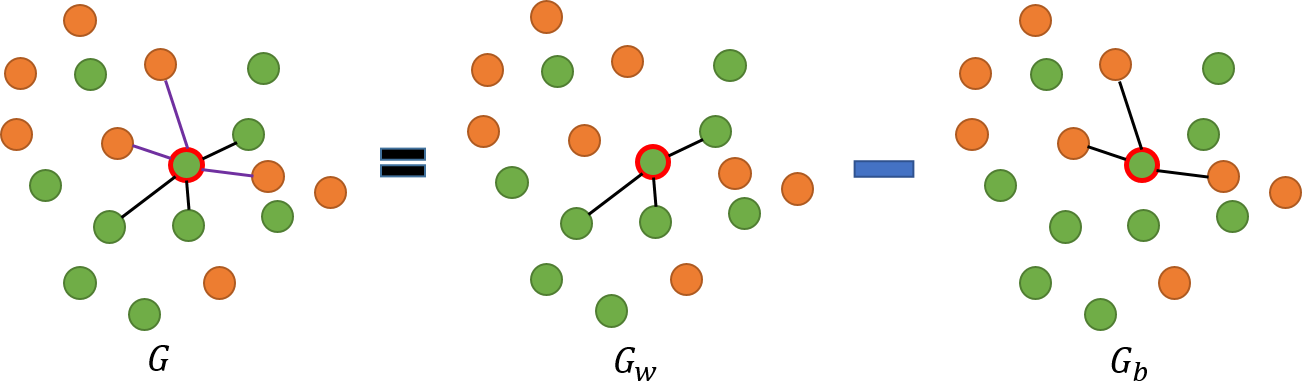
\includegraphics[width=\linewidth]{source/Graph_Embedding.png}
	\caption{图嵌入框架示意图}
	\label{fig:Graph_Embedding}
\end{figure}
此外,为了平衡正负样本对的比例,实验中还将$G$中的$1,-1$分别除以正负样本对的个数。

接下来,使用$\rho_{ij}=\frac{\left<Z_{i},Z_{j}\right>_{F}}{\|Z_{i}\|_{F}\|Z_{j}\|_{F}};i,j=1,2,\cdots n$来度量两个表示之间的相似度\footnote{注:这里不使用$\frac{\left<Z_{i}^{\frac{1}{m}},Z_{j}^{\frac{1}{m}}\right>_{F}}{\|Z_{i}\|_{F}^{\frac{1}{m}}\|Z_{j}^{\frac{1}{m}}\|_{F}};i,j=1,2,\cdots n$的原因主要是这会大大增加计算复杂度而且当$n>1$时$x^{\frac{1}{n}}$的导数未定义,所以这里退而求其次};利用$\rho_{ij}$和$G_{ij}$的定义,给出公式\ref{FRPSD_discriminant}中的损失函数:
\begin{equation}
\label{FRPSD_discriminant}
C(Z)=-\sum_{i=1}^{n}\sum_{j=1}^{n}G_{ij}\rho_{ij}^{2}={\rm tr}(GF^{T})+\gamma\|Z\|_{F}^{2},where~F_{ij}=\rho_{ij}^{2}
\end{equation}
其中函数$C(Z)$的最后一项是正则项,其目的是为了防止过拟合,这虽然只是一个小的trick,但是实验中发现该trick却比较有效。

我们的目标是使最终编码的$Z_{i}, i=1,2,\cdots n$让$C(Z)$最小。这是一个矩阵函数的优化问题,为此需要计算目标函数的导数。为了叙述的方便,这里把第二章的两条在计算矩阵方向导数的时候的规律($rule$\ref{devi_rules_2})再表述一遍。
\begin{displaymath}
\label{devi_rules}
\left\{
\begin{split}
&rule~1:D_{X}(f\circ g)(X)[H]=D_{g(X)}f(g(X))[D_{X}g(X)[H]]\\
&rule~2:D_{X}\left<f(X),g(X)\right>[H]=\left<D_{X}f(X)[H],g(X)\right>+\left<f(X),D_{X}g(X)[H]\right>
\end{split}
\right.
\end{displaymath}
关于矩阵函数的方向导数的具体内容,读者可以参看本文第二章的内容,此外读者也可以在\cite{Maniopt_DiscreteCurveFitting}中找到关于$rule~1,rule~2$的内容。

对于最小化问题\ref{FRPSD_discriminant},这里使用共轭梯度算法进行求解,为此需要预先计算$C(Z)$的梯度$\nabla_{Z}C(Z)$,为了方便起见定义$k_{ij}=\left<Z_{i},Z_{j}\right>_{F}$,接下来利用公式\ref{discrimZ_search_gradeint}对$C(Z)$计算其关于$Z$的导数。
\begin{equation}
\label{discrimZ_search_gradeint}
\begin{split}
C(Z)={\rm tr}(GF^{T})+\gamma\|Z\|_{F}^{2}&=\sum_{i=1}^{n}\sum_{j=1}^{n}G_{ij}F_{ij}+\gamma\|Z\|_{F}^{2}=\sum_{i=1}^{n}\sum_{j=1}^{n}G_{ij}\frac{k_{ij}^2}{k_{ii}k_{jj}}+\gamma\|Z\|_{F}^{2}\\
\frac{\partial}{\partial Z}C(Z)&=\sum_{i=1}^{n}\sum_{j=1}^{n}G_{ij}\left(c_1\frac{\partial}{\partial Z}k_{ij}-c_2\frac{\partial}{\partial Z}k_{ii}-c_3\frac{\partial}{\partial Z}k_{jj}\right)+2\gamma Z\\
{\rm where~~}c_1&=\frac{2k_{ij}k_{ii}k_{jj}}{(k_{ii}k_{jj})^2},c_2=\frac{k_{ij}k_{ij}k_{jj}}{(k_{ii}k_{jj})^2},c_3=\frac{k_{ij}k_{ij}k_{ii}}{(k_{ii}k_{jj})^2}
\end{split}
\end{equation}
公式\ref{discrimZ_search_gradeint}中$\frac{\partial}{\partial Z}k_{ij}$的计算与第二章中第一个例子\ref{MatrixFunc_devi_example1}的计算类似,具体过程如下:
\begin{equation}
\label{discrimZ_search_part1_gradeint}
\begin{split}
D_{Z}k_{ij}[H]&=D_{Z}\left<Z_i,Z_j\right>_{F}\\
&=\left<D_{Z}Z_i[H],Z_j\right>_{F}+\left<Z_i,DZ_j[H]\right>_{F}
\end{split}
\end{equation}
由于$\left<D_{Z}Z_i[H],Z_j\right>_{F}$与$\left<Z_i,D_{Z}Z_j[H]\right>_{F}$的计算是类似的,所以仅以前一部分作为研究对象,其结果可以很好的平移到另一部分。
\begin{equation}
\label{discrimZ_search_part2_gradeint}
\begin{split}
\left<D_{Z}Z_i[H],Z_j\right>_{F}&=\left<D_{Z}\left((C_{i}^{\frac{1}{2}}+Z)S_{i}(C_{i}^{\frac{1}{2}}+Z)^{T}\right)[H],(C_{j}^{\frac{1}{2}}+Z)S_{j}(C_{j}^{\frac{1}{2}}+Z)^{T}\right>_{F}\\
D_{Z}\left((C_{i}^{\frac{1}{2}}+Z)S_{i}(C_{i}^{\frac{1}{2}}+Z)^{T}\right)[H]&=D_{Z}(C_{i}^{\frac{1}{2}}S_{i}C_{i}^{\frac{T}{2}}+C_{i}^{\frac{1}{2}}S_{i}Z^{T}+ZS_{i}C_{i}^{\frac{T}{2}}+ZS_{i}Z^{T})[H]\\
&=C_{i}^{\frac{1}{2}}S_{i}H^{T}+HS_{i}C_{i}^{\frac{T}{2}}+HS_{i}Z^{T}+ZS_{i}H^{T}\\
&=(C_{i}^{\frac{1}{2}}+Z)S_{i}H^{T}+HS_{i}(C_{i}^{\frac{T}{2}}+Z^{T})
\end{split}
\end{equation}
其中$S_{i}=Y_{i}Y_{i}^{T},i=1,2,\cdots,n$,接下来利用公式\ref{discrimZ_search_part2_gradeint}的结果,得到公式\ref{discrimZ_gradient}的结果(其中利用了$Z_{i},S_{i};i=1,2,\cdots,n$是对称矩阵的结果)。
\begin{equation}
\label{discrimZ_gradient}
\left\{
\begin{split}
\left<D_{Z}Z_i[H],Z_j\right>_{F}&=\left<(C_{i}^{\frac{1}{2}}+Z)S_{i}H^{T}+HS_{i}(C_{i}^{\frac{T}{2}}+Z^{T}),Z_j\right>_{F}\\
&={\rm tr}\left((C_{i}^{\frac{1}{2}}+Z)S_{i}H^{T}Z_j\right)+{\rm tr}\left(HS_{i}(C_{i}^{\frac{T}{2}}+Z^{T})Z_j\right)\\
&={\rm tr}\left(H^{T}Z_j(C_{i}^{\frac{1}{2}}+Z)S_{i}\right)+{\rm tr}\left(HS_{i}(C_{i}^{\frac{T}{2}}+Z^{T})Z_j\right)\\
&=2{\rm tr}\left(H^{T}Z_j(C_{i}^{\frac{1}{2}}+Z)S_{i}\right)=2\left<H,Z_j(C_{i}^{\frac{1}{2}}+Z)S_{i}\right>_{F}\\
D_{Z}k_{ij}[H]&=2\left<H,Z_j(C_{i}^{\frac{1}{2}}+Z)S_{i}\right>_{F}+2\left<H,Z_i(C_{j}^{\frac{1}{2}}+Z)S_{j}\right>_{F}\\
\frac{\partial}{\partial Z}k_{ij}&=2Z_j(C_{i}^{\frac{1}{2}}+Z)S_{i}+2Z_i(C_{j}^{\frac{1}{2}}+Z)S_{j}\\
&=2(Z_{j}W_{i}Y_{i}^{T}+Z_{i}W_{j}Y_{j}^{T})
\end{split}
\right.
\end{equation}
最后结合公式\ref{discrimZ_search_gradeint}和\ref{discrimZ_gradient}的结果,即可计算出$C(Z)$的梯度,将其作为共轭梯度算法的输入,最小化$C(Z)$获得$Z^{*}$即可用于对图像集合的PSD编码。这里使用图\ref{fig:Discrim_LRPSD}示意带判别信息的低秩对称正定矩阵编码图像集合的模型。
\begin{figure}[htb]
	\centering
	\subcaptionbox{半正定矩阵平方根示意图}
      	{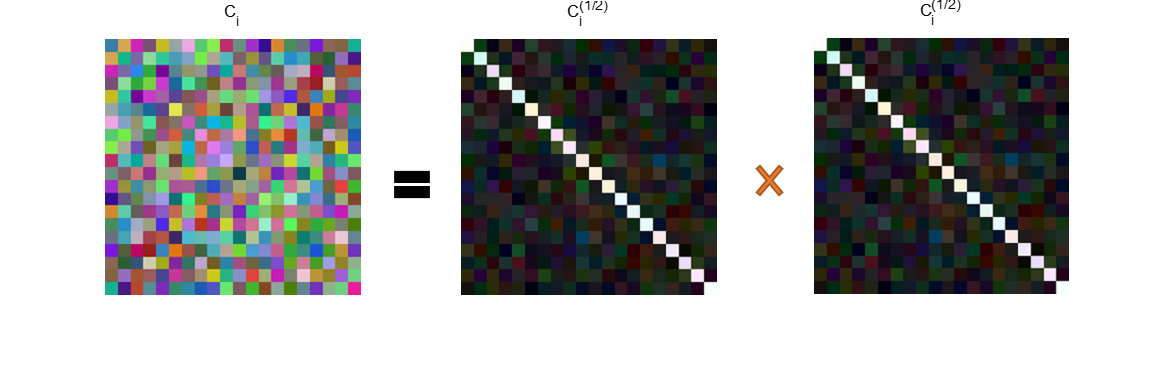
\includegraphics[width=\linewidth]{source/Discrim_LRPSD_sqrt.png}}
	\subcaptionbox{编码判别信息的$W_{i}$的示意图}
		{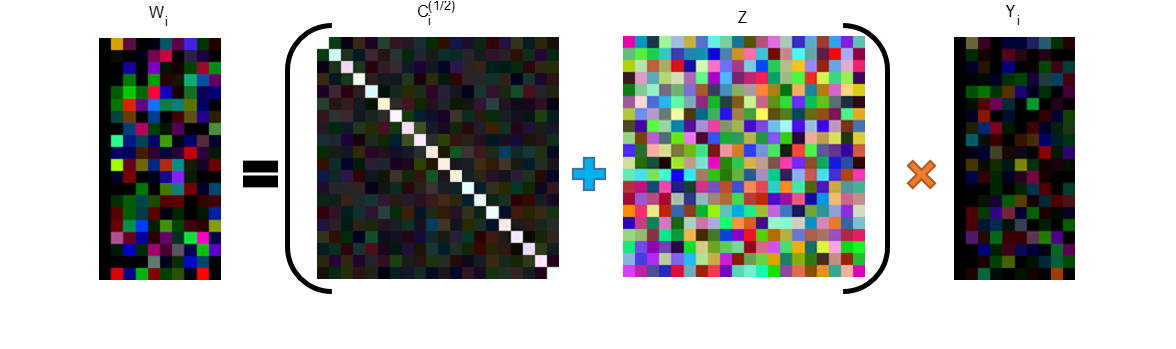
\includegraphics[width=\linewidth]{source/Discrim_LRPSD_W.png}}
	\caption{带判别信息的低秩对称半正定矩阵模型示意图}
	\label{fig:Discrim_LRPSD}
\end{figure}
\subsection{低秩对称半正定矩阵集合上的判别学习方法}
在\ref{sec:discrim_Low_Rank_PSD}小节中介绍了将判别信息编码到Low-Rank PSD矩阵问题,但是仅仅有内嵌入判别性的编码还是不足以处理太复杂的问题,且算法也不具有Large Margin等性质,类似于\cite{PSD_WACV}中的方法,这里选择在核判别学习(Kernel Discriminant Learning, KDA\cite{Kernel_KDA})的框架下进行判别学习。特别地,注意到Power-Euclidean度量的定义可以由$k_{ij}=\left<Z_{i}^{\frac{1}{m}},Z_{j}^{\frac{1}{m}}\right>_{F}$的kernel的形式导出,并且容易证明$K=\{k_{ij}\}_{n\times  n}$的正定性。

由于KDA\cite{Kernel_KDA}的研究已经非常成熟,且这里也不是对它的改进或相关的工作,所以不会从头再介绍一遍,而只会简单的回顾一下KDA的基本思想:首先,KDA的基础是线性判别分析(Linear Discriminant Analysis, LDA),其目标是使得内类散度小而类间散度大。KDA则是LDA在再生核希尔伯特空间(Reproducing Kernel Hilbert space, RKHS)中的版本,其目的与LDA一样。文献\cite{Kernel_KDA}中给出了十分简洁的KDA的形式:设$n_c,c=1,2,\cdots,C$表示各个类别中的样本数,$\sum_{c=1}^{C}n_{c}=n$,这里的$n$表示的是样本总数,$\phi(\cdot)$表示的是非线性变化(例如接下来将要使用的$\phi(Z_{i})=Z_{i}^{\frac{1}{n}},n>1$),定义核矩阵$K=\{k_{ij}\}_{n\times n}$,其中$k_{ij}=\left<\phi(Z_{i}),\phi(Z_j)\right>_{F}$,则KDA的目标形式化为公式\ref{KDA_Formulation}。
\begin{equation}
\label{KDA_Formulation}
\bm{\alpha}_{opt}=\arg \max\frac{\bm{\alpha}^{T}KWK\bm{\alpha}}{\bm{\alpha}^{T}KK\bm{\alpha}}
\end{equation}
其中$W$的定义如公式\ref{KDA_W_def}所示。
\begin{equation}
\label{KDA_W_def}
W=\{W_{ij}\}_{n \times n},\text{where }W_{ij}=\left\{
\begin{split}
&\frac{1}{n_{c}},\text{若$Z_{i},Z_{j}$同时属于第c类}\\
&0, \text{否则}
\end{split}
\right.
\end{equation}
以上便是本章所提方法使用的判别学习方法——KDA\cite{Kernel_KDA}的介绍,试验中我们使用了文献\cite{KDA_DengCai1,KDA_DengCai2}提供的代码。
\section{实验结果与分析}
本章所做的问题是使用Low-Rank PSD矩阵表示集合数据,并在该表示下进行集合数据的分类问题,任务与第二章的任务类似,都是集合数据的分类问题,所以这里使用了相同的数据进行实验(物体识别数据库ETH\cite{Database_ETH80},材质分类数据库UIUC\cite{Database_UIUC}以及视频人脸识别数据库\cite{Database_YTC}),这几个数据库上的实验任务已经在\ref{sec:RPLS_exp}部分做了相对细致的介绍,同时数据库的规模(包含了小数据库ETH,中等规模数据库UIUC,较大规模的数据库YTC)也具有一定的代表性;各个数据集合上的基本特征的提取与\ref{Database_feature}节介绍的方式相同,这里不再赘述;在获得原始特征之后,利用公式\ref{MeanCov_SPD_Construct}构造初始半正定矩阵表示$C_{i}$(此时不需要再加正则项),然后利用\ref{sec:discrim_Low_Rank_PSD}的编码过程获得图像集合带判别性的低秩对称半正定矩阵表示。关于数据库的详细介绍以及对应的测试协议可以参看\ref{sec:data_intro}部分的内容,而关于原始图像特征的提取部分的内容则可以参看\ref{Database_feature}节的内容。最后表\ref{tab:LRPSD_experiment}给出了我们的实验结果。

\begin{table}[htb]
	\centering
	\caption{低秩对称半正定矩阵判别学习方法对比实验结果}
	\begin{tabular*}{\linewidth}{@{\extracolsep{\fill}}|l|ccc|}\hline
		\diagbox{方法}{数据集} &ETH80 &UIUC &YTC \\ \hline
		GDA\cite{Subspace_GDA} &92.50$\pm$3.54	&53.33$\pm$2.32 &66.73$\pm$3.16 \\ \hline
		CDL-PLS\cite{Statistics_CDL} &93.25$\pm$4.72 &53.89$\pm$4.06 &70.28$\pm$2.13 \\ \hline
		RSR-Stein\cite{Dictionary_RSR} &93.25$\pm$3.34 &52.41$\pm$4.03 &72.77$\pm$2.69  \\ \hline
		SPDML-Stein\cite{Statistics_SPDML} &90.50$\pm$3.87 &49.17$\pm$2.37 &61.57$\pm$3.43  \\ \hline
		SPDML-AIM\cite{Statistics_SPDML} &90.75$\pm$3.34 &48.09$\pm$1.82 &64.66$\pm$2.92  \\ \hline
		LEML\cite{Statistics_LEML}&94.75$\pm$2.49 &48.98$\pm$3.69 &70.53$\pm$2.95  \\ \hline
		${\rm FRPSD-KDA}_{Linear}$\cite{PSD_WACV}&94.50$\pm$3.07	&52.04$\pm$3.80	&70.93$\pm$3.28  \\ \hline
		${\rm FRPSD-KDA}_{Polynomial}$\cite{PSD_WACV}&\textbf{96.00$\pm$2.42}	&56.02$\pm$3.93 &70.74$\pm$3.05  \\ \hline
		${\rm FRPSD-KDA}_{Laplace}$\cite{PSD_WACV}&95.50$\pm$2.84 &57.69$\pm$3.35 &70.14$\pm$3.04  \\ \hline
		${\rm FRPSD-KDA}_{RBF}$\cite{PSD_WACV}&95.50$\pm$3.50 &57.78$\pm$4.10 &70.96$\pm$3.05\\ \hline
		${\rm \bm{LRPSD-KDA}}$ &\textbf{93.25$\pm$4.72} &\textbf{59.17$\pm$3.48} &\textbf{74.37$\pm$2.96}  \\ \hline
		${\rm \bm{LRPSD-KDA}}_{discrim}$ &\textbf{94.50$\pm$2.48} &\textbf{59.81$\pm$3.58} &\textbf{74.73$\pm$2.91}  \\ \hline
	\end{tabular*}
	\label{tab:LRPSD_experiment}
\end{table}
其中,${\rm FRPSD-KDA}$是文章\cite{PSD_WACV}中方法的简称(是Fixed-Rank PSD和KDA的缩写),其下标表示了核的类型:线性核($Linear$)、多项式核($Polynomial$)、Laplace核($Laplace$)以及RBF核($RBF$),${\rm LRPSD-KDA}$则表示本章所提的方法的简称(是Low-Rank PSD和KDA的缩写),其中下标$discrim$表示的方法是否使用\ref{sec:discrim_Low_Rank_PSD}部分的编码学习方式构造图像集合的Low-Rank PSD矩阵表示。

表格\ref{tab:LRPSD_experiment}中选取的方法与\ref{sec:RPLS_exp_result_analysis}部分选择方法类似,包含了目前取得state-of-the-art的一些主要方法,此外还包含了与我们最相关的工作\cite{PSD_WACV}中的方法的结果,由于作者没有公布源代码,所以我们小心的实现并进行细致的参数调节之后汇报我们所获得的最好的结果。还有GDA\cite{Subspace_GDA}的结果(该结果也是自己实现并小心调参后获得的结果)。其它方法我们均从作者主页获取代码并小心调参后汇报的最好的结果。

从表格\ref{tab:LRPSD_experiment}我们的可以得到的信息是:本章所提的${\rm \bm{LRPSD-KDA}}$方法在三个数据集上获得了与state-of-the-art可比甚至是更好的性能,相较于子空间和协方差建模的方法(表格\ref{tab:LRPSD_experiment}的前两行),${\rm \bm{LRPSD-KDA}}$方法在三个任务上都有相对明显的提升。我们认为获得这种提升的主要原因有两个方面:1)通过与文章\cite{PSD_WACV}中的方法(表中的${\rm FRPSD-KDA}$一类方法)相比,可得出本文使用的Power-Euclidean度量更能刻画PSD矩阵的性质的结论,这与我们的一开始的想法是吻合的;2)表中的最后六行的结果与其它行的结果相比说明了PSD建模图像集合的有效性。最后还注意到融入判别信息带来提升,虽然幅度不大(这与本文选择的相对简单的融合方式有关)但是可以看出方向的正确性,这里还有上升的空间。

实验中还发现:公式\ref{FRPSD_discriminant}中的正则项$\gamma\|Z\|_{F}^{2}$对结果的影响与数据集相关,对于每个集合中数据较少或噪声较大的数据集,如ETH\cite{Database_ETH80}和YTC\cite{Database_YTC}(其中YTC属于集合个数多,但是每个集合都不是很大的类型,这在视频监控中很常见)该项的设置很重要,但是对于每个集合中样本较多的数据集该项则可忽略掉(如:在UIUC\cite{Database_UIUC}上我们设置$\gamma=0$),其它实验参数的设置主要包含$k_w,k_b$的设置,Power-Euclidean度量中$n$(或$\alpha=\frac{1}{n}$)的设置,以及Low-Rank约束的上界$k$的设置。由于都是整数设置方法比较常规这里就不再一一赘述。最后,需要注意的是利用Power-Euclidean度量还可以定义其它的核的形式,表\ref{tab:PSD_PowerMetric_KernelList}中给出了kernel的形式:
\begin{table}[htb]
  \centering
  \begin{minipage}[t]{0.8\linewidth} % 如果想在表格中使用脚注,minipage是个不错的办法
  \caption{Power-Euclidean度量相关的核}
  \label{tab:PSD_PowerMetric_KernelList}
    \begin{tabular*}{\linewidth}{lp{10cm}}
      \toprule[1.5pt]
      {\heiti 名称} & {\heiti 形式化} \\\midrule[1pt]
      线性核 & $k_{l}(A,B)={\rm tr}\left(Z_{i}^{\frac{1}{m}}Z_{j}^{\frac{T}{m}}\right)$\\
      多项式核 & $k_{p}(A,B)=\left(\beta+{\rm tr}\left(Z_{i}^{\frac{1}{m}}Z_{j}^{\frac{T}{m}}\right)\right)^{\alpha}$\\
      拉普拉斯核 & $k_{L}(A,B)=\exp\left(-\beta\sqrt{\|Z_{i}^{\frac{1}{m}}-Z_{j}^{\frac{T}{m}}\|_{F}^{2}}\right)$\\
      RBF核 & $k_{R}(A,B)=\exp\left(-\beta{\|Z_{i}^{\frac{1}{m}}-Z_{j}^{\frac{T}{m}}\|_{F}^{2}}\right)$\\
      \bottomrule[1.5pt]
    \end{tabular*}
  \end{minipage}
\end{table}

但是从实验结果中可以看出:在线性核下我们已经得到了与state-of-the-art可比甚至是更好一些的结果,此外Kernel的方法的引入虽然会对最终的结果有所提高(部分测试试验中发现Laplace Kernel对于Power-Euclidean度量有更好的促进作用),但是由于引入了更多的参数需要调节,所以使得算法的实际运用价值打了折扣;因此这里仅把kernel的方法作为一个未来深入方向,而不在这里做深入讨论。
\section{总结与下一步工作}
在本章中我们针对集合数据的建模问题以及集合数据特征本身存在的一些问题,使用PSD矩阵建模图像集合,并且结合前期关于Fixed-Rank PSD流形的研究以及工作\cite{PSD_WACV}的内容,针对使用子空间、协方差矩阵以及Fixed-Rank PSD矩阵建模图像集合的工作\cite{PSD_WACV}中存在的问题,提出了Low-Rank PSD矩阵的判别学习方法,主要的内容可以归纳为如下几点:1)使用带有判别性的低秩对称半正定矩阵表示图像集合;2)针对文献\cite{PSD_WACV}中的使用的$\delta_{FRPSD}(\cdot,\cdot)$(公式\ref{polar_metric})割裂了Grassmann流形和对称正定矩阵流形之间关系的问题提出了使用Power-Euclidean度量进行判别学习的方法;3)在KDA\cite{Kernel_KDA}的框架下进行判别学习获得与state-of-the-art可比甚至是更好的结果。

最后,前面已经提到表格\ref{tab:LRPSD_experiment}中的结果显示判别学习与非判别学习的结果提升不是特别的明显,究其原因的话可能是Graph Embedding的框架与最后的KDA的框架没有很好的适配的原因,这里的问题值得深入研究,此外就是前面提到的使用更多Kernel版本的方法,可能也是一个尝试的方向。